\documentclass[11pt,letterpaper]{article}
\usepackage[margin=0.85in,headheight=14pt]{geometry}
\usepackage{amsmath,amssymb}
\usepackage{enumitem}
\usepackage{fancyhdr}
\usepackage{lmodern}
\usepackage[T1]{fontenc}
\usepackage[dvipsnames]{xcolor}
\usepackage[most]{tcolorbox}
\usepackage{pgfplots}
\usepgfplotslibrary{groupplots,fillbetween}
\usetikzlibrary{arrows.meta,positioning,shapes.geometric,calc,decorations.pathreplacing}
\pgfplotsset{
  compat=1.18,
  every axis/.append style={grid=major, grid style={gray!25}, tick label style={font=\footnotesize},
    label style={font=\small}, title style={font=\small}, legend style={font=\scriptsize}},
}
\definecolor{cA}{HTML}{1F77B4}
\definecolor{cB}{HTML}{FF7F0E}
\definecolor{cC}{HTML}{2CA02C}
\definecolor{cD}{HTML}{D62728}
\definecolor{cE}{HTML}{9467BD}

\pagestyle{fancy}
\fancyhf{}
\lhead{SYDE 556/750 \qquad Test 2}
\rhead{Solutions \& marking guide}
\cfoot{\thepage}
\renewcommand{\headrulewidth}{0pt}

\setlength{\parindent}{0pt}
\setlength{\parskip}{4pt}

\newcommand{\tref}{\tau_{\mathrm{ref}}}
\newcommand{\trc}{\tau_{RC}}
\newcommand{\T}{\mathsf T}
\newcommand{\Jb}{J^{\mathrm{bias}}}
\newcommand{\ans}[1]{\par\vspace{4pt}{\bfseries #1}\quad}

\newtcolorbox{marking}{colback=blue!3,colframe=blue!40!black,boxrule=0.4pt,left=4pt,right=4pt,top=2pt,bottom=2pt,arc=1pt,fonttitle=\bfseries\small,title=Marking}
\newtcolorbox{trap}{colback=red!4,colframe=red!50!black,boxrule=0.4pt,left=4pt,right=4pt,top=2pt,bottom=2pt,arc=1pt,fonttitle=\bfseries\small,title=Where marks are usually lost}

\begin{document}

\begin{center}
{\Large\bfseries Test 2: Temporal Representation \& Feedforward Transformations --- Solutions}\\[2pt]
Total: 20 marks plus 2 bonus. Simulation data: \texttt{tests\_data/make\_data.py}.\\
Mark splits are inferred from the marked paper where possible.
\end{center}

%=====================================================================
\section*{Question 1 \hfill (4)}

\ans{(a) [2]}
\begin{enumerate}[leftmargin=1.6em, label=\arabic*.]
\item \textbf{Frequency grid.} With time step $\Delta t$, use $N = T/\Delta t$ samples. The discrete frequencies are $\omega_k = 2\pi k/T$.
\item \textbf{Sample the band.} For every $0 < |\omega_k| \le 2\pi L$, draw $X(\omega_k) = a + ib$ with $a, b \sim \mathcal N(0, 1)$. Set every other coefficient to $0$, including $\omega = 0$ (zero mean).
\item \textbf{Make it real.} Set $X(-\omega_k) = X^*(\omega_k)$ (see (b)).
\item \textbf{Back to time and rescale.} Take the inverse FFT, $x(t) = \mathcal F^{-1}[X]$. Then rescale, $x \leftarrow x \cdot \sigma/\mathrm{RMS}(x)$, so that the RMS is exactly $\sigma$.
\end{enumerate}
\begin{marking}
0.5 each: grid or band in rad/s ($2\pi L$), random complex coefficients inside the band and zero outside, symmetry, inverse FFT \emph{and} rescale to RMS $\sigma$. A low-pass ``smoothing filter'' in place of the inverse FFT and rescale loses the last half-mark.
\end{marking}

\ans{(b) [1]}
\[
X(-\omega) = X^*(\omega),
\]
so the real part is even and the imaginary part is odd, and $X(0)$ must be real. Each pair $\pm\omega$ then sums to a real cosine with a phase, $2|X|\cos(\omega t + \phi)$. The lecture notes write this loosely as ``$X(\omega) = X(-\omega)$''. The conjugate is the precise statement.

\ans{(c) [1]}
On average $|X(\omega)|$ is \textbf{flat} (white) inside the band and zero outside. On an angular-frequency axis the edges are at $\omega = \pm 2\pi L$. On an axis in Hz they are at $\pm L$.
\begin{center}
\begin{tikzpicture}
\begin{groupplot}[group style={group size=2 by 1, horizontal sep=1.5cm}, height=4.6cm]
\nextgroupplot[width=0.52\textwidth, xmin=-75, xmax=75, ymin=0, ymax=1.25,
  xlabel={$\omega$ (rad/s)}, ylabel={average $|X(\omega)|$ (normalized)},
  title={400 signals, $L = 5$ Hz}, xtick={-62.8,-31.4,0,31.4,62.8},
  xticklabels={$-4\pi L$,$-2\pi L$,$0$,$2\pi L$,$4\pi L$}]
  \addplot[cA, very thick, const plot mark mid] table[x expr=2*pi*\thisrow{f}, y=mag] {tests_data/t2q1_spectrum.dat};
  \draw[cD, dashed, thick] (axis cs:-31.4,0) -- (axis cs:-31.4,1.2);
  \draw[cD, dashed, thick] (axis cs:31.4,0) -- (axis cs:31.4,1.2);
  \node[cD, font=\scriptsize, anchor=south west] at (axis cs:31.4,1.05) {$\omega = 2\pi L$};
\nextgroupplot[width=0.48\textwidth, xmin=0, xmax=2, ymin=-1.5, ymax=1.5,
  xlabel={$t$ (s)}, ylabel={$x(t)$}, title={One sample, RMS $\sigma = 0.5$}]
  \addplot[cA, thick] table[x=t, y=x] {tests_data/t2q1_signal.dat};
\end{groupplot}
\end{tikzpicture}
\end{center}
The dip at $\omega = 0$ comes from setting $X(0) = 0$ (zero mean).
\begin{marking}
0.5: flat inside the band, zero outside, symmetric about $0$. \ 0.5: axes labelled and the cutoff marked at $\pm 2\pi L$ on a $\omega$ axis (or $\pm L$ on a Hz axis). Writing $\pm L$ on an axis labelled $\omega$ loses this half-mark.
\end{marking}

%=====================================================================
\section*{Question 2 \hfill (4)}
\begin{itemize}[leftmargin=1.2em]
\item $v$: the (normalized) \textbf{membrane voltage}. The threshold is $1$ and the reset value is $0$.
\item $J$: the (normalized) \textbf{input current} into the soma, in the same units, so $J = 1$ is the threshold current.
\item $\trc = RC$: the \textbf{membrane time constant}, from the membrane's capacitance $C$ and leak resistance $R$. It sets how fast $v$ moves.
\item $dv/dt$: the rate of change of the voltage. The $-v$ term is the \textbf{leak}: charge drains out at a rate proportional to $v$.
\end{itemize}
\textbf{The whole equation} is a leaky integrator (an RC circuit). The voltage charges up and relaxes exponentially toward $J$ with time constant $\trc$: from $v(0) = 0$, $v(t) = J(1 - e^{-t/\trc})$.
\begin{itemize}[leftmargin=1.2em]
\item If $J \le 1$, $v$ settles at $J$ below threshold and the neuron never fires.
\item If $J > 1$, $v$ reaches the threshold $1$ after $t_{\mathrm{th}} = -\trc\ln(1 - 1/J)$. At threshold the neuron \textbf{emits a spike}, $v$ is \textbf{reset to $0$} and \textbf{held there for the refractory period $\tref$}, and then integration restarts.
\end{itemize}
This repeats with period $\tref + t_{\mathrm{th}}$, which gives the rate $G[J] = \bigl(\tref - \trc\ln(1 - 1/J)\bigr)^{-1}$. The plot below uses $\trc = 20$ ms and $\tref = 2$ ms, with $J$ stepping from $0$ to $1.5$ at $t = 10$ ms.
\begin{center}
\begin{tikzpicture}
\begin{axis}[width=0.92\textwidth, height=5.4cm, xmin=0, xmax=100, ymin=-0.05, ymax=1.85,
  xlabel={$t$ (ms)}, ylabel={$v(t)$}, legend style={at={(0.5,1.02)}, anchor=south}, legend cell align=left, legend columns=3]
  \addplot[cA, very thick] table[x=t, y=v] {tests_data/t2q2_voltage.dat};
  \addplot[cB, thick, dashed] table[x=t, y=J] {tests_data/t2q2_voltage.dat};
  \addplot[cD, thick, densely dotted, domain=0:100, samples=2] {1};
  \legend{$v(t)$, $J(t)$, threshold}
  \foreach \s in {31.9,55.9,79.9} {
    \edef\tmp{\noexpand\fill[gray!35] (axis cs:\s,-0.05) rectangle (axis cs:\s+2,1.0);}\tmp
    \edef\tmp{\noexpand\draw[black, thick] (axis cs:\s,1) -- (axis cs:\s,1.6);}\tmp
  }  \draw[{Stealth}-{Stealth}] (axis cs:10,1.15) -- node[above, font=\scriptsize] {$t_{\mathrm{th}} = \trc\ln 3 \approx 22$ ms} (axis cs:31.9,1.15);
  \node[font=\scriptsize, anchor=west, align=left] at (axis cs:58.2,0.3) {reset to $0$,\\held for $\tref$};
  \node[font=\scriptsize, anchor=south] at (axis cs:55.9,1.6) {spike};
\end{axis}
\end{tikzpicture}
\end{center}
\begin{marking}
0.5 each for $v$, $J$, $\trc$, and $dv/dt$ (2). \ 1: leaky integration toward $J$ (RC circuit), including no spikes when $J \le 1$. \ 1: at threshold, spike, \emph{reset to $0$}, and \emph{refractory period $\tref$}. Missing the reset or refractory period loses half a mark.
\end{marking}

%=====================================================================
\section*{Question 3 \hfill (4)}

\ans{(a) [2]}
The normalization is $c = \int_0^\infty t^n e^{-t/\tau}dt = n!\,\tau^{n+1}$.
\begin{itemize}[leftmargin=1.2em]
\item $n = 0$: $h(t) = \frac1\tau e^{-t/\tau}$. This is the exponential synapse. It jumps to its maximum $1/\tau$ \textbf{at $t = 0$} and then decays.
\item $n = 1$: $h(t) = \frac{t}{\tau^2}e^{-t/\tau}$. This is the alpha synapse. It \textbf{starts at $0$}, rises to a peak of $1/(e\tau) \approx 0.37/\tau$ at $t = \tau$, and has a longer tail.
\end{itemize}
Both have unit area.
\begin{center}
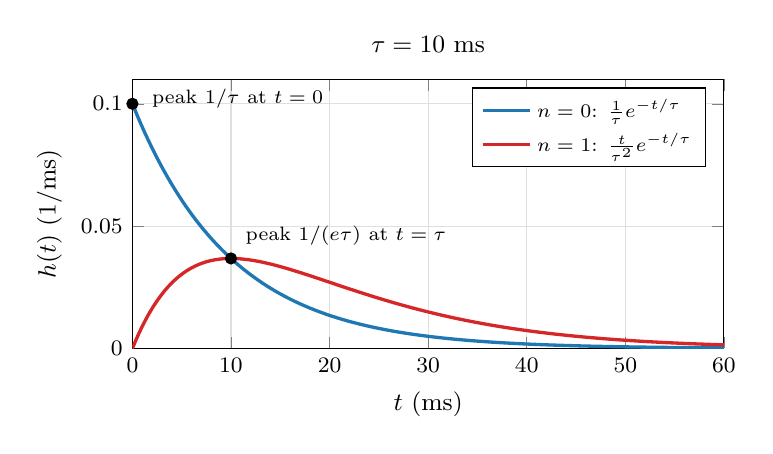
\begin{tikzpicture}
\begin{axis}[width=0.75\textwidth, height=5cm, xmin=0, xmax=60, ymin=0, ymax=0.11,
  xlabel={$t$ (ms)}, ylabel={$h(t)$ (1/ms)}, legend pos=north east, legend cell align=left,
  title={$\tau = 10$ ms}, scaled y ticks=false, yticklabel style={/pgf/number format/fixed}]
  \addplot[cA, very thick, domain=0:60, samples=200] {exp(-x/10)/10};
  \addplot[cD, very thick, domain=0:60, samples=200] {x*exp(-x/10)/100};
  \legend{$n = 0$: $\frac1\tau e^{-t/\tau}$, $n = 1$: $\frac{t}{\tau^2}e^{-t/\tau}$}
  \addplot[only marks, mark=*, black] coordinates {(0,0.1) (10,0.0368)};
  \node[font=\scriptsize, anchor=west] at (axis cs:1,0.102) {peak $1/\tau$ at $t = 0$};
  \node[font=\scriptsize, anchor=south west] at (axis cs:10.5,0.038) {peak $1/(e\tau)$ at $t = \tau$};
\end{axis}
\end{tikzpicture}
\end{center}
\begin{marking}
1: $n = 0$ curve has its maximum at $t = 0$ and decays monotonically. \ 1: $n = 1$ curve starts at $0$, peaks later (at $t = \tau$), and is lower and wider.
\end{marking}

\ans{(b) [2]}
A larger $\tau$ is a lower cut-off low-pass filter (cut-off $\approx 1/(2\pi\tau)$ Hz). Two effects on $\hat x(t)$:
\begin{enumerate}[leftmargin=1.6em, label=\arabic*.]
\item \textbf{Smoother.} Spike noise (the ripple from individual spikes) is averaged over a longer window, so $\hat x$ is less noisy.
\item \textbf{More delayed and sluggish.} $\hat x$ lags $x$ and responds more slowly to fast changes. Fast signal components are attenuated.
\end{enumerate}
\begin{center}
\begin{tikzpicture}
\begin{axis}[width=0.92\textwidth, height=5.6cm, xmin=0, xmax=2, ymin=-3, ymax=3,
  xlabel={$t$ (s)}, ylabel={$\hat x(t)$}, legend style={at={(0.5,1.02)}, anchor=south}, legend cell align=left, legend columns=3]
  \addplot[cB, thin, opacity=0.6] table[x=t, y=tau5] {tests_data/t2q5_decode.dat};
  \addplot[cA, very thick] table[x=t, y=tau50] {tests_data/t2q5_decode.dat};
  \addplot[black, dashed, thick] table[x=t, y=x] {tests_data/t2q5_decode.dat};
  \legend{$\tau = 5$ ms, $\tau = 50$ ms, $x(t)$}
\end{axis}
\end{tikzpicture}
\end{center}
This uses the two LIF neurons from Question~5, decoded with the $n = 0$ filter. With $\tau = 50$ ms the trace is much smoother, but it is visibly shifted right (for a $1$ Hz sine the lag is about $\arctan(2\pi \cdot 0.05)/2\pi \approx 48$ ms).
\begin{marking}
1 each: smoother or less noisy; more delay or lag (slower response to changes). ``Lower amplitude for fast signals'' also earns the second mark.
\end{marking}

%=====================================================================
\section*{Question 4 \hfill (4)}

\ans{(a) [1]}
\begin{itemize}[leftmargin=1.2em]
\item \textbf{Function decoders on $P_1$} for $f(x) = 2x + 1$:
$\mathbf D^{f} = \bigl((\mathbf A\mathbf A^\T + N\sigma^2\mathbf I)^{-1}\mathbf A\mathbf Y^\T\bigr)^\T$, with $\mathbf Y = f(\mathbf X)$ evaluated at the sample points.
\item \textbf{Identity decoders on $P_2$} (target $y$), to read out the final $\hat y$.
\end{itemize}
The $+1$ is affine, so identity decoders on $P_1$ with a transform of $2$ cannot produce it alone. Either decode $2x + 1$ directly or add a constant input. Also, if $x \in [-1, 1]$ then $y \in [-1, 3]$, so $P_2$ needs a radius of about $3$.

\ans{(b) [3]}
\begin{enumerate}[leftmargin=1.6em, label=\arabic*.]
\item \textbf{Encode into $P_1$.} The input $x$ becomes a current in each neuron: $J_i = \alpha_i\langle e_i, x\rangle + \Jb_i$.
\item \textbf{$P_1$ nonlinearity.} Each neuron spikes: $a_i(t) = G_i[J_i(t)]$.
\item \textbf{Decode $f$ from $P_1$.} The spikes are filtered by the synapse and weighted by the function decoders: $\hat y = \sum_i d^{f}_i\,(h * a_i) \approx 2x + 1$.
\item \textbf{Encode into $P_2$.} $J_j = \alpha_j\langle e_j, \hat y\rangle + \Jb_j$. Steps 3 and 4 together are the weight matrix $\omega_{ji} = \alpha_j\langle e_j, d^{f}_i\rangle$.
\item \textbf{$P_2$ nonlinearity.} $b_j(t) = G_j[J_j(t)]$.
\item \textbf{Decode the output.} Filter $P_2$'s spikes and apply its identity decoders: $\hat y = \sum_j d_j\,(h * b_j)$.
\end{enumerate}
\begin{center}
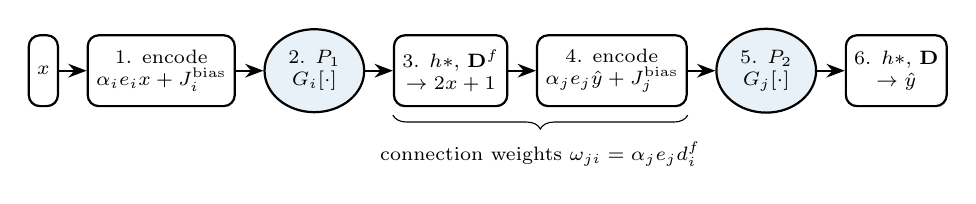
\begin{tikzpicture}[font=\scriptsize, node distance=0.35cm,
  box/.style={draw, thick, rounded corners, align=center, minimum height=0.9cm, inner sep=3pt},
  pop/.style={draw, thick, ellipse, align=center, minimum height=0.9cm, fill=cA!10}]
  \node[box] (x) {$x$};
  \node[box, right=of x] (e1) {1. encode\\$\alpha_i e_i x + \Jb_i$};
  \node[pop, right=of e1] (p1) {2. $P_1$\\$G_i[\cdot]$};
  \node[box, right=of p1] (d1) {3. $h *$, $\mathbf D^{f}$\\$\to 2x + 1$};
  \node[box, right=of d1] (e2) {4. encode\\$\alpha_j e_j \hat y + \Jb_j$};
  \node[pop, right=of e2] (p2) {5. $P_2$\\$G_j[\cdot]$};
  \node[box, right=of p2] (d2) {6. $h *$, $\mathbf D$\\$\to \hat y$};
  \foreach \a/\b in {x/e1, e1/p1, p1/d1, d1/e2, e2/p2, p2/d2} \draw[-{Stealth}, thick] (\a) -- (\b);
  \draw[decorate, decoration={brace, amplitude=5pt, mirror}] (d1.south west) ++(0,-0.1) -- ($(e2.south east)+(0,-0.1)$)
    node[midway, below=6pt] {connection weights $\omega_{ji} = \alpha_j e_j d^{f}_i$};
\end{tikzpicture}
\end{center}
\begin{marking}
(a) 0.5: function decoders for $2x + 1$ on $P_1$. \ 0.5: identity decoders on $P_2$ for the output. \ (b) 0.5 per step, in the correct order (encode, nonlinearity, decode with filter, twice).
\end{marking}

%=====================================================================
\section*{Question 5 \hfill (4)}
Same $\alpha$ and $\Jb$ with opposite encoders gives mirror-image tuning curves. Neuron 1 fires only when $x$ is above its intercept, and neuron 2 only when $x$ is below the mirrored intercept. In the simulation below the intercepts are at $0$ and $a^{\max} = 60$ Hz.
\begin{itemize}[leftmargin=1.2em]
\item \textbf{Spike trains.} Neuron 1 fires during the positive half-cycles, with the \textbf{highest spike density at the peaks} ($x = +1$) and sparse spikes near the zero crossings. Neuron 2 does the same during the negative half-cycles, densest at the troughs. Neither fires near $x = 0$.
\item \textbf{Decoded signal.} With $d_2 = -d_1$, each neuron-1 spike adds a filtered bump of $+d_1$ and each neuron-2 spike adds one of $-d_1$. $\hat x(t)$ follows the sine in shape and size, but it is \textbf{noisy}: a sawtooth ripple from individual spikes. It is slightly \textbf{delayed} by the synapse.
\end{itemize}
\begin{center}
\begin{tikzpicture}
\begin{groupplot}[group style={group size=1 by 3, vertical sep=0.35cm, xticklabels at=edge bottom},
  width=0.92\textwidth, xmin=0, xmax=2]
\nextgroupplot[height=3.2cm, ymin=-1.2, ymax=1.2, ylabel={$x(t)$}]
  \addplot[black, very thick] table[x=t, y=x] {tests_data/t2q5_decode.dat};
\nextgroupplot[height=2.8cm, ymin=0.4, ymax=2.6, ytick={1,2}, yticklabels={$e_1 = +1$, $e_2 = -1$}, ylabel={spikes}, grid=none]
  \addplot[cA, only marks, mark=|, mark size=7pt, thick] table[x=t, y expr=1] {tests_data/t2q5_spikes1.dat};
  \addplot[cD, only marks, mark=|, mark size=7pt, thick] table[x=t, y expr=2] {tests_data/t2q5_spikes2.dat};
\nextgroupplot[height=4.2cm, ymin=-1.6, ymax=1.6, ylabel={$\hat x(t)$}, xlabel={$t$ (s)},
  legend style={at={(0.5,-0.45)}, anchor=north}, legend cell align=left, legend columns=2]
  \addplot[cC, thick] table[x=t, y=tau20] {tests_data/t2q5_decode.dat};
  \addplot[black, dashed] table[x=t, y=x] {tests_data/t2q5_decode.dat};
  \legend{$\hat x$ ($\tau = 20$ ms), $x$}
\end{groupplot}
\end{tikzpicture}
\end{center}
\begin{marking}
1: sine input over a couple of periods. \ 1: each neuron fires only in its own half-cycle. \ 0.5: spike density increases toward the peak or trough (rate code). \ 1: $\hat x$ tracks the sine and is drawn as a noisy, rippled reconstruction rather than a clean sine. \ 0.5: slight delay, or near-zero output where neither neuron fires.
\end{marking}
\begin{trap}
Drawing evenly spaced spikes (the rate must follow $|x|$), or drawing $\hat x$ as a perfect sine. Two neurons give a very rough estimate.
\end{trap}

%=====================================================================
\section*{Bonus Question 1 \hfill (2)}
$H(\omega)$ is the least-squares (Wiener) filter. It is the linear filter $h$ for which $\hat x = h * r$ is as close as possible to $x$. At each frequency it acts like a regression coefficient:
\[
H(\omega) = \frac{\text{cross-spectrum (covariance) of signal and response}}{\text{power spectrum (variance) of the response}}.
\]
\begin{itemize}[leftmargin=1.2em]
\item \textbf{Numerator} $\langle X R^*\rangle$: how strongly, and with what phase, the response at frequency $\omega$ is correlated with the signal. Spike power that is unrelated to the signal averages out to about zero over many trials or windows.
\item \textbf{Denominator} $\langle |R|^2\rangle$: the total response power at $\omega$, both signal-related and spike noise. Dividing by it normalizes the gain. Frequencies where the response is mostly spike noise get a small gain, and frequencies where the response reliably tracks the signal get a large one.
\end{itemize}
The phase of $H$ corrects for the delay between signal and spikes, so $h(t)$ is generally \textbf{non-causal} (nonzero for $t < 0$). The lecture's windowed version smooths both spectra in frequency, which gives a smoother, shorter $h(t)$.
\begin{center}
\begin{tikzpicture}
\begin{groupplot}[group style={group size=2 by 1, horizontal sep=1.5cm}, height=5cm]
\nextgroupplot[width=0.44\textwidth, xmin=-150, xmax=150, xlabel={$t$ (ms)}, ylabel={$h(t)$},
  title={Optimal filter (windowed, 60 trials)}, scaled y ticks=false, yticklabel style={/pgf/number format/fixed}]
  \addplot[cA, very thick] table[x=t, y=h] {tests_data/t2b_filter.dat};
  \draw[gray, dashed] (axis cs:0,-0.05) -- (axis cs:0,0.2);
\nextgroupplot[width=0.56\textwidth, xmin=0, xmax=2, ymin=-1.6, ymax=1.6, xlabel={$t$ (s)}, ylabel={$x$},
  title={Held-out test signal ($L = 5$ Hz)}, legend pos=south east, legend cell align=left, legend columns=2]
  \addplot[black, dashed, thick] table[x=t, y=x] {tests_data/t2b_decode.dat};
  \addplot[cC, thick] table[x=t, y=xhat] {tests_data/t2b_decode.dat};
  \legend{$x$, $\hat x = h * r$}
\end{groupplot}
\end{tikzpicture}
\end{center}
Here $r = s_1 - s_2$ is the signed spike train of the two neurons from Question~5.
\begin{marking}
1: the filter finds the linear filter that minimizes the squared decoding error, by correlating input with response across frequencies. \ 1: numerator is the signal--response cross-correlation (cross-spectrum), and the denominator normalizes by the response power, so noise-dominated frequencies are suppressed.
\end{marking}

\end{document}
